\documentclass[a4paper]{article}

\usepackage[portuguese]{babel}
\usepackage[utf8]{inputenc}
\usepackage{graphicx,hyperref}
\usepackage{float}
\usepackage{listings}
\usepackage{proof,tikz}
\usepackage{algorithm2e}
\usepackage{amssymb,amsthm,stmaryrd}


\usepackage[edges]{forest}
\usetikzlibrary{automata, positioning, arrows}


\newtheorem{Lemma}{Lema}
\newtheorem{Theorem}{Teorema}
\theoremstyle{definition}
\newtheorem{Example}{Exemplo}
\newtheorem{Definition}{Definição}
\newtheorem{Fact}{Fato}


\usepackage{fancyhdr}
  \pagestyle{fancy}
  \fancyhf{}
  \lhead{Teoria da Computação}
  \rhead{Aula 26}
  \lfoot{Prof. Rodrigo Ribeiro}
  \rfoot{\thepage}
  \renewcommand{\footrulewidth}{0.4pt}
  \pagestyle{fancy}

\tikzset{
        ->,  % makes the edges directed
        >=stealth', % makes the arrow heads bold
        node distance=3cm,
        every state/.style={thick, fill=gray!10},
        initial text=$\,$
        }
  

\begin{document}

\title{Aula 26 - O Problema de Correspondência de Post}
  \author{Rodrigo Ribeiro}

  \maketitle

  \pagestyle{fancy}


  \section*{Objetivos}

  \begin{itemize}
    \item Apresentar a prova de indecidibilidade do problema de correspondência
      de Post (PCP).
  \end{itemize}


  \section{Introdução}

  O objetivo desta aula é apresentar a prova de indecibilidade do PCP, que é um
  problema simples sobre palavras de um certo alfabeto. A utilidade do PCP vem
  do fato que este pode ser utilizado para demonstrar a indecibilidade de
  diversos problemas de cunho ``mais prático'', como por exemplo, problemas
  relativos a gramáticas livres de contexto - que são utilizadas para descrever
  a sintaxe de linguagens de programação - e também a inexistência de
  estratégias para sempre vencer no jogo Tetris.


  \section{O Problema de Correspondência de Post}

  \begin{Definition}
    Um sistema de correspondência de Post (SCP) é um par $(\Sigma,P)$, em que
    $P$ é uma sequência finita de pares $(x,y)$ tais que $x,y\in \Sigma^+$.
  \end{Definition}

  Uma solução para um SCP $S = (\Sigma,P)$ é uma sequência de pares de $P$ tal
  que a palavra formada pela concatenação dos primeiros elementos dos pares
  é igual a palavra formada pela concatenação dos segundos elementos dos
  mesmos pares. A seguir definimos esse conceito formalmente.

  \begin{Definition}
    Seja um SCP $S = (\Sigma, [(x_1,y_1),...,(x_n,y_n)])$. Uma solução para $S$
    é uma sequência $i_1,...,i_k$ tal que
    \[
      x_{i1}x_{i2}...x_{ik} = y_{i1}y_{i2}...y_{ik}
    \]
    para $1 \leq i_j \leq n$ para $1 \leq j \leq k$.
  \end{Definition}

  Antes de apresentar a prova de indecidibilidade do PCP, vamos considerar um
  exemplo.

  \begin{Example}
    Seja o SCP $(\{0,1\}, [(10,0), (0,010), (01,11)])$. Esse SCP possui três
    pares: $(x_1 = 10, y_1 = 0)$, $(x_2 = 0, y_2 010)$ e $(x_3 = 01, y_3 = 11)$.
    Uma possível solução para esse SCP seria a sequência 2131. Fica mais fácil
    visualizar a solução representando pares como frações. Por exemplo,
    representamos o par $(10,0)$ por $\frac{10}{0}$. Dessa forma, usando os
    índices 2131 obtemos:
    \[
      \begin{array}{cccc}
        \frac{0}{010} &
        \frac{10}{0}  & 
        \frac{01}{11} &
        \frac{10}{0}
      \end{array}
    \]
    Evidentemente, repetições da sequência 2131 também formam soluções.
    Exemplos: 21312131, 2131213121312131, etc.
  \end{Example}

  O problema de decisão a ser mostrado indecidível consiste em determinar se um
  SCP qualquer possui solução. Para isso, vamos introduzir um problema
  intermediário para facilitar a prova de indecidibilidade a partir do problema
  da parada. A figura a seguir ilustra as reduções a serem feitas.

  \begin{figure}[H]
    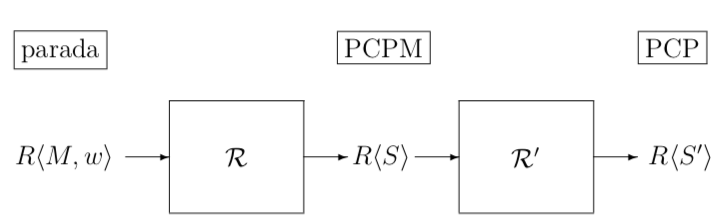
\includegraphics[scale=.35]{reductions.png}
    \centering
  \end{figure}

  O problema intermediário é conhecido como problema de correspondência de Post
  modificado e é definido a seguir.

  \begin{Definition}
    O problema de correspondência de Post modificado (PCPM) consiste em
    determinar se um PCP arbitrário tem solução iniciada com o índice 1.
  \end{Definition}

  \begin{Example}
    Seja o SCP $(\{0,1\}, [(0,010), (10,0), (01,11)])$. Esse SCP possui solução
    para o PCPM e esta é: 1232.
  \end{Example}

  Agora vamos demonstrar a primeira parte da redução: que o PCPM é redutível ao
  PCP.

  \begin{Theorem}
    O PCPM é redutível ao PCP
  \end{Theorem}
  \begin{proof}
    Seja um SCP $S = (\Sigma, P)$ com $P = [(x_1,y_1),...,(x_n,y_n)]$. Sejam
    ``\#'' e ``*'' símbolos não pertencentes a $\Sigma$. Considere:
    \begin{itemize}
      \item $x'_i$ o resultado de colocar um ``*'' depois de cada símbolo de
        $x_i$. Por exemplo, se $x_i = 010$ então $x'_i = 0*1*0*$.
      \item $y'_i$ o resultado de colocar um ``*'' antes de cada símbolo de
        $y_i$. Por exemplo, se $y_i = 100$ então $y'_i = *1*0*0$.
     \end{itemize}
     Seja o SCP $S' = (\Sigma\cup\{*,\#\},P')$ em que $P'$ é formado pelos
     pares:
     \begin{itemize}
        \item $(*x'_1,y_1)$, o primeiro par da solução.
        \item $(x'_i,y'_i)$, para $1\leq i \leq n$.
        \item $(\#,*\#)$.
     \end{itemize}
     Agora, basta mostrar que se $S'$ tem solução então $S$ também tem. Suponha
     que $S'$ possui solução. Note que o único par de $S'$ que começa com o
     mesmo símbolo é $(*x'_1, y'_1)$ e o único que termina com o mesmo símbolo é
     $(\#,*\#)$. Dessa forma, a solução para $S'$ deve ser da forma:
     \[
       \begin{array}{cccc}
         \frac{*x'_1}{y'_1} &
         ...                & 
         \frac{x'_{i_k}}{y'_{i_k}} & 
         \frac{\#}{*\#}
       \end{array}
     \]
     Ora, dessa forma, removendo o último par e todos os ``*'' presentes em cada
     $x'_i,y'_i$ obtemos uma solução para o PCP a partir de uma do PCPM.
  \end{proof}

  Para concluir a indecidibilidade do PCP, vamos mostrar como reduzir a entrada
  do problema da parada para o PCPM. A idéia da redução é construir pares do
  PCPM de forma que cada par represente as possíveis configurações que a MT
  passa durante sua computação com a palavra $w$. Os pares são construídos de
  forma que o PCPM possui solução se, e somente se, a MT $M$ para com a palavra
  $w$.

  \begin{Theorem}
    O PCPM é indecidível.
  \end{Theorem}
  \begin{proof}
    Seja $M = (E,\Sigma,\Gamma,\langle, \sqcup,\delta,i,F)$ uma MT e $w \in
    \Sigma^*$ uma palavra. A partir destas construiremos um SCP $S =
    (\Delta,P)$, em que:
    \begin{itemize}
      \item $\Delta = \Sigma \cup \{*,\#\}$;
      \item O primeiro elemento de $P$ é $(*,*\langle iw*)$
      \item Os demais pares de $P$ são:
        \begin{itemize}
          \item $(c,c)$ para cada $c \in \Gamma$;
          \item $(*,*)$;
          \item Para cada $a,b \in \Gamma$ e $e,e' \in E$:
            \[
              \begin{array}{l}
                (ea,be'), \textit{se }\delta(e,a) = [e',b,D]\\
                (e*,be'*), \textit{se }\delta(e,\sqcup) =[e',b,D]\\
                (cea,e'cb), \textit{se }\delta(e,a) = [e',b,E],\textit{ para
                cada }c\in\Gamma\\
                (ce*,e'cb*),\textit{se }\delta(e,\sqcup) = [e',b,E],\textit{
                para cada }c\in\Gamma.\\
              \end{array}
            \]
          \item $(ea,\#)$, se $\delta(e,a) = \bot$, para cada $e\in E$ e $a
            \in\Gamma$;
          \item $(e*,\#*)$, se $\delta(e,\sqcup) = \bot$, para cada $e\in E$.
          \item $(c\#,\#)$, para cada $c \in \Gamma$.
          \item $(\#c,\#)$, para cada $c \in\Gamma$.
          \item $(* \# *, *)$.
        \end{itemize}
      \end{itemize}
      Pode-se mostrar que $M$ para com entrada $w$, se e somente se, o $SCP$ $S$
      tiver solução iniciada com $(*,*\langle iw*)$.
    \end{proof}

    \begin{Example}
      Considere a seguinte MT que aceita $1(0+1)^*$:
      \begin{figure}[H]
        \begin{tikzpicture}[node distance=3cm]
          \node[state, initial, accepting](s0){$A$};
          \node[state, right of=s0](s1){$B$};
          \draw (s0)edge[above]node{$0/0\:D$}(s1) ;
        \end{tikzpicture}
        \centering
      \end{figure}
      O SCP correspondente a $M$ e a palavra $11$ é formado pelos seguintes
      pares:
      \begin{itemize}
         \item $(*,*\langle A11*)$, que corresponde ao primeiro par.
         \item $(\langle, \langle)$, $(\sqcup,\sqcup)$, $(0,0)$ , $(1,1)$ e
           $(*,*)$.
         \item A transição $\delta(A,0) = [B,0,D]$ produz o par:
           $(A0,0B)$.
         \item Como $\delta(A,1) = \delta(A,\langle) = \delta(A,\sqcup) = \bot$,
           temos os seguintes pares: $(A1,\#)$, $(A\langle, \#)$ e $(A\sqcup,\#)$.
         \item Como $\delta(A,\sqcup) = \bot$, temos o par $(A*,\#*)$.
         \item Como $\delta(B,0) = \delta(B,1) = \delta(B,\langle) =
           \delta(B,\sqcup) = \bot$, temos os seguintes pares: $(B0,\#)$,
           $(B1,\#)$, $(B\langle,\#)$, $(B\sqcup,\#)$.
         \item Como $\delta(B,\sqcup) = \bot$, temos: $(B*,\#*)$.
         \item Incluir os pares para cada símbolo de $\Gamma$: $(\langle\#,\#)$,
           $(\sqcup\#,\#)$, $(0\#,\#)$ e $(1\#,\#)$.
         \item Incluir os pares $(\#\langle,\#)$, $(\#\sqcup,\#)$, $(\#0,\#)$ e
           $(\#1,\#)$.
         \item Incluir o par $(*\# *,*)$.
      \end{itemize}
    \end{Example}

    A partir do PCP, prodemos provar a indecidibilidade de diversos problemas
    envolvendo gramáticas livres de contexto. Esse será o assunto da próxima aula.
\end{document}
